\documentclass[11pt,a4paper]{article}
\usepackage[main=italian,provide=*]{babel}
\usepackage[utf8]{inputenc}
\usepackage[T1]{fontenc}
\usepackage{amsmath,amssymb}
\usepackage{geometry}
\geometry{margin=2.7cm}
\usepackage{booktabs}
\usepackage{array}
\usepackage{caption}
\usepackage{multirow}
\usepackage{tikz}
\usepackage[colorlinks=true,linkcolor=blue,citecolor=blue]{hyperref}

\title{Simmetria e Antisimmetria nell'Hamiltoniana di Scambio tra Due Spin 1/2:\\
dal Modello di Heisenberg all'Interazione di Dzyaloshinskii--Moriya\\[6pt]
\large Appunti di meccanica quantistica dello spin}
\author{}
\date{20 luglio 2026}

\begin{document}
\maketitle

\begin{abstract}
\noindent Questo documento raccoglie in forma organica lo studio delle propriet\`a di
simmetria e antisimmetria di un'Hamiltoniana di scambio tra due spin 1/2. La Parte~I
tratta il sistema isolato: si parte dalla definizione dell'operatore di permutazione
$P_{12}$ e dalla distinzione tra la componente simmetrica dell'interazione (il modello
di Heisenberg isotropo) e quella antisimmetrica (l'interazione di
Dzyaloshinskii--Moriya, DMI); si analizzano la struttura degli stati di singoletto e
tripletto, il ruolo fisico del segno della costante di scambio $J$, il meccanismo per
cui la DMI mescola singoletto e tripletto, l'effetto di tale mescolamento sulle
degenerazioni energetiche, l'inclinazione (canting) degli spin e la diagonalizzazione
esatta per un vettore $\vec D$ generico. La Parte~II va oltre il sistema isolato:
discute l'origine microscopica di $J$ e $\vec D$ (superscambio e regole di Moriya),
l'anisotropia di scambio come meccanismo -- fisicamente corretto per spin 1/2 -- per
rimuovere la degenerazione residua, un esempio numerico di ordini di grandezza
realistici, la mappatura della DMI su operatori di Pauli rilevante per il calcolo
quantistico, e alcuni cenni sull'estensione a pi\`u spin e alla chiralit\`a nelle
strutture ad anello.
\end{abstract}

\tableofcontents

\section{Introduzione}

La simmetria o antisimmetria di un'Hamiltoniana per scambio di spin definisce come
varia l'energia del sistema quando si invertono le posizioni (gli indici) di due spin.
In generale:
\begin{itemize}
\item la simmetria indica che l'Hamiltoniana resta invariata sotto l'azione
dell'operatore di scambio, $[H,P_{12}]=0$;
\item l'antisimmetria si riferisce invece a specifici termini energetici -- come
l'interazione di Dzyaloshinskii--Moriya -- che cambiano segno quando i due spin vengono
scambiati di posto.
\end{itemize}
Questi due comportamenti non sono soltanto una curiosit\`a formale: determinano la
geometria delle configurazioni magnetiche permesse al sistema, dividendo il problema in
una parte che favorisce l'allineamento collineare (parallelo o antiparallelo) e una
parte che, al contrario, favorisce configurazioni non collineari, inclinate o chirali.

\section{Notazione}

Per fissare le convenzioni usate nel seguito:
\begin{itemize}
\item \textbf{Operatori a scala.} Per ciascun sito $i$ si definiscono $S_i^\pm =
S_{ix}\pm iS_{iy}$, con $S_i^+|\!\downarrow\rangle=|\!\uparrow\rangle$,
$S_i^-|\!\uparrow\rangle=|\!\downarrow\rangle$, e azione nulla oltre gli stati
estremali (spin 1/2).
\item \textbf{Stati di spin totale.} Con $\vec S=\vec S_1+\vec S_2$, gli stati
$|S,M\rangle$ sono autostati simultanei di $\vec S^2$ (autovalore $S(S+1)$) e di
$S_z=S_{1z}+S_{2z}$ (autovalore $M$); sono legati alla base computazionale
$\{|\!\uparrow\uparrow\rangle,|\!\uparrow\downarrow\rangle,|\!\downarrow\uparrow\rangle,|\!\downarrow\downarrow\rangle\}$
dalle combinazioni di Clebsch--Gordan per due spin 1/2 riportate nelle sezioni
seguenti.
\item \textbf{Elementi di matrice.} Si scrive $\langle a|O|b\rangle$ per l'elemento di
matrice dell'operatore $O$ tra gli stati $|a\rangle$ e $|b\rangle$.
\item \textbf{Legame con gli operatori di Pauli.} Per spin 1/2 vale $\vec S_i =
\tfrac12\vec\sigma_i$, dove $\vec\sigma_i=(X_i,Y_i,Z_i)$ sono le matrici di Pauli sul
sito $i$; questa relazione sar\`a usata nella Parte~II per la mappatura su qubit.
\end{itemize}

\part{Il sistema isolato: simmetria di Heisenberg e antisimmetria di Dzyaloshinskii--Moriya}

\section{L'operatore di scambio}

Per descrivere matematicamente lo scambio di due spin si introduce l'operatore di
permutazione (o di scambio) $P_{12}$. Se i due spin occupano le posizioni 1 e 2 con
operatori vettoriali $\vec S_1$ e $\vec S_2$, l'azione di $P_{12}$ consiste nello
scambiare i loro indici:
$$P_{12}\,\vec S_1\,P_{12}^{-1}=\vec S_2, \qquad P_{12}\,\vec S_2\,P_{12}^{-1}=\vec S_1.$$
L'operatore $P_{12}$ \`e unitario ed hermitiano, con $P_{12}^\dagger=P_{12}$ e
$P_{12}^2=I$: applicarlo due volte riporta il sistema allo stato di partenza. \`E
proprio l'effetto di $P_{12}$ sull'Hamiltoniana completa a determinare se il sistema
possiede propriet\`a di simmetria o antisimmetria per scambio.

\section{Scambio simmetrico: il modello di Heisenberg}

Si parla di simmetria per scambio quando l'Hamiltoniana complessiva commuta con
l'operatore di scambio:
$$[H,P_{12}]=0 \;\Longrightarrow\; P_{12}HP_{12}^{-1}=H.$$
Questo significa che scambiare lo spin 1 con lo spin 2 non altera l'energia del
sistema.

\paragraph{Esempio classico.} Il modello di Heisenberg isotropo, in cui l'interazione
\`e proporzionale al prodotto scalare dei due spin,
$$H_{\rm sym}=J\,\vec S_1\cdot\vec S_2,$$
\`e l'esempio paradigmatico di questa simmetria. Poich\'e il prodotto scalare \`e
commutativo, $\vec S_1\cdot\vec S_2=\vec S_2\cdot\vec S_1$, scambiare l'ordine degli
spin non modifica l'espressione dell'energia.

\paragraph{Effetto fisico.} Il sistema favorisce un allineamento collineare: parallelo
se l'accoppiamento \`e ferromagnetico ($J<0$), antiparallelo se \`e antiferromagnetico
($J>0$). Gli autostati dell'Hamiltoniana si dividono in stati simmetrici (i tripletti)
e antisimmetrici (il singoletto) rispetto allo scambio.

\section{Scambio antisimmetrico: l'interazione di Dzyaloshinskii--Moriya}

L'antisimmetria per scambio si riferisce invece a una componente dell'Hamiltoniana che
cambia segno matematico quando gli indici dei due spin vengono invertiti:
$$H_{\rm antisym}(1,2)=-H_{\rm antisym}(2,1).$$

\paragraph{Esempio classico.} L'interazione di Dzyaloshinskii--Moriya (DMI), espressa
tramite un prodotto vettoriale,
$$H_{\rm DMI}=\vec D_{12}\cdot(\vec S_1\times\vec S_2),$$
realizza esattamente questa antisimmetria. Poich\'e il prodotto vettoriale \`e
anticommutativo, $\vec S_1\times\vec S_2=-(\vec S_2\times\vec S_1)$, affinch\'e
l'energia totale resti fisicamente coerente il vettore di Dzyaloshinskii--Moriya deve a
sua volta essere antisimmetrico rispetto allo scambio dei siti: $\vec D_{12}=-\vec
D_{21}$.

\paragraph{Effetto fisico.} Questa interazione si manifesta nei sistemi privi di
simmetria di inversione cristallina. Non potendo azzerarsi l'energia con un
allineamento collineare, la DMI favorisce un allineamento perpendicolare o inclinato
(canted) degli spin, dando origine a strutture magnetiche complesse come i vettori
chirali, le onde di spin elicoidali o i cristalli di skyrmioni.

\section{Confronto tra i due comportamenti}

\paragraph{Conclusione parziale.} La simmetria per scambio implica che l'Hamiltoniana
non varia invertendo i due spin, favorendo configurazioni magnetiche collineari;
l'antisimmetria indica invece che l'Hamiltoniana cambia segno sotto inversione dei siti
a causa di accoppiamenti vettoriali, favorendo configurazioni magnetiche inclinate o
chirali.

\begin{center}
\begin{tabular}{@{}p{3.1cm}p{4.9cm}p{4.9cm}@{}}
\toprule
Caratteristica & Scambio simmetrico & Scambio antisimmetrico (DMI) \\
\midrule
Operazione matematica & Prodotto scalare $\vec S_1\cdot\vec S_2$ & Prodotto vettoriale $\vec D\cdot(\vec S_1\times\vec S_2)$ \\
Comportamento per scambio & Invariato ($+H$) & Cambio di segno ($-H$) \\
Configurazione geometrica & Collineare (parallelo/antiparallelo) & Non collineare (perpendicolare/inclinata) \\
Origine fisica & Interazione di scambio quantistico diretta & Accoppiamento spin-orbita in assenza di inversione \\
\bottomrule
\end{tabular}

\captionof{table}{Confronto tra la componente simmetrica (Heisenberg) e antisimmetrica (DMI) dell'Hamiltoniana di scambio.}
\end{center}

\section{Stati di singoletto e tripletto nel caso collineare}

Quando \`e favorito un allineamento collineare, come nel modello di Heisenberg, lo
stato fondamentale del sistema dipende dal segno della costante di accoppiamento $J$.
\`E importante notare che la distinzione tra singoletto e tripletto non si limita al
valore del numero quantico magnetico $M$ (la proiezione lungo l'asse $z$), ma riguarda
lo spin totale $S$ dei due elettroni.

\subsection{Caso antiparallelo: antiferromagnetismo ($J>0$)}

Quando il sistema favorisce un allineamento antiparallelo, lo stato a energia minima
(fondamentale) \`e il singoletto di spin ($S=0$, $M=0$), sovrapposizione quantistica
antisimmetrica
$$|S=0,M=0\rangle=\frac1{\sqrt2}\big(|\!\uparrow\downarrow\rangle-|\!\downarrow\uparrow\rangle\big).$$
In questo stato gli spin sono strettamente opposti. Lo stato di tripletto con $M=0$,
$\tfrac1{\sqrt2}(|\!\uparrow\downarrow\rangle+|\!\downarrow\uparrow\rangle)$, ha invece
la stessa energia degli stati con $M=\pm1$ e si trova a un'energia pi\`u alta (stato
eccitato).

\subsection{Caso parallelo: ferromagnetismo ($J<0$)}

Quando il sistema favorisce un allineamento parallelo, lo stato fondamentale \`e il
tripletto di spin ($S=1$), tre volte degenere, che comprende tutti e tre gli stati:
\begin{align}
|S=1,M=1\rangle &= |\!\uparrow\uparrow\rangle, \\
|S=1,M=-1\rangle &= |\!\downarrow\downarrow\rangle, \\
|S=1,M=0\rangle &= \frac1{\sqrt2}\big(|\!\uparrow\downarrow\rangle+|\!\downarrow\uparrow\rangle\big).
\end{align}
Il ruolo dello stato $M=0$ nel tripletto merita un commento: sebbene a livello
microscopico, nella base computazionale, $|\!\uparrow\downarrow\rangle$ e
$|\!\downarrow\uparrow\rangle$ sembrino antiparalleli, la loro combinazione lineare
simmetrica (il tripletto $M=0$) descrive in realt\`a spin che sono paralleli nel piano
trasversale $xy$. Pertanto questo stato mantiene le stesse propriet\`a energetiche e di
simmetria degli stati totalmente paralleli $M=\pm1$.

\subsection{Confronto riassuntivo}

Se l'allineamento favorito \`e antiparallelo si ottiene dunque il singoletto ($S=0$,
$M=0$); se \`e parallelo si ottiene l'intero tripletto ($S=1$), che include sia gli
stati puramente paralleli ($M=\pm1$) sia lo stato simmetrico con $M=0$.

\begin{center}
\begin{tabular}{@{}p{3.6cm}p{2.2cm}p{3cm}p{4cm}@{}}
\toprule
Allineamento favorito & Segno di $J$ & Stato fondamentale & Valori di $M$ del fondamentale \\
\midrule
Antiparallelo (antiferromagnetico) & $J>0$ & Singoletto ($S=0$) & solo $M=0$ \\
Parallelo (ferromagnetico) & $J<0$ & Tripletto ($S=1$) & tutti e tre: $M=+1,0,-1$ \\
\bottomrule
\end{tabular}
\captionof{table}{Stato fondamentale collineare in funzione del segno di $J$.}
\end{center}

\section{Il ruolo fisico del segno della costante $J$}

Pu\`o essere utile un'interpretazione intuitiva del parametro $J$: esso pu\`o essere
pensato come una manopola che stabilisce la regola del gioco tra due spin. L'energia di
interazione si scrive schematicamente come
$$E = J\cdot(\text{orientazione degli spin}).$$
Poich\'e ogni sistema fisico tende verso lo stato di energia pi\`u bassa possibile,
\`e il segno di $J$ a decidere quale configurazione, parallela o antiparallela,
risulti energeticamente favorita.
\begin{itemize}
\item Se $J>0$: la formula dell'energia premia l'allineamento opposto. Lo stato
antiparallelo ha energia minima, e il sistema sceglie il singoletto ($M=0$).
\item Se $J<0$: il segno negativo inverte la regola, premiando l'allineamento
concorde. Il sistema sceglie la configurazione parallela, descritta dal tripletto
(che include sia il parallelismo perfetto $M=\pm1$ sia la combinazione simmetrica
$M=0$).
\end{itemize}
In sintesi: l'Hamiltoniana collineare stabilisce soltanto che gli spin si disporranno
sullo stesso asse; \`e il valore di $J$ a stabilire in che verso, concorde o discorde,
essi si orienteranno.

\subsection{Verifica esplicita tramite il prodotto scalare}

Il motivo per cui l'energia sale o scende in funzione dell'orientazione pu\`o essere
reso esplicito applicando la semplice regola dei segni al prodotto scalare $\vec
S_1\cdot\vec S_2$ dell'Hamiltoniana di scambio $H=J(\vec S_1\cdot\vec S_2)$.
Sostituendo le frecce di spin con numeri orientati lungo l'asse $z$
($\uparrow\to+1$, $\downarrow\to-1$), si ottengono i due casi seguenti.

\paragraph{Spin paralleli ($\uparrow\uparrow$).} Il prodotto dei segni \`e positivo,
$(+1)(+1)=+1$: per $J>0$ l'energia risulta positiva (alta); per $J<0$ risulta negativa
(bassa).

\paragraph{Spin antiparalleli ($\uparrow\downarrow$).} Il prodotto dei segni \`e
negativo, $(+1)(-1)=-1$: per $J>0$ l'energia risulta negativa (bassa); per $J<0$
risulta positiva (alta).

Poich\'e i sistemi fisici cercano sempre lo stato di energia pi\`u bassa possibile,
\`e questo semplice gioco dei segni a decidere matematicamente quale delle due
geometrie costa meno e viene quindi selezionata dagli spin.

\begin{center}
\begin{tabular}{@{}p{4.8cm}p{2.8cm}p{1.6cm}p{4cm}@{}}
\toprule
Regime & Configurazione & Energia & Esito \\
\midrule
$J>0$ (antiferromagnetico) & Paralleli & $+J$ & alta \\
$J>0$ (antiferromagnetico) & Antiparalleli & $-J$ & bassa, fondamentale (singoletto) \\
$J<0$ (ferromagnetico) & Paralleli & $-J$ & bassa, fondamentale (tripletto) \\
$J<0$ (ferromagnetico) & Antiparalleli & $+J$ & alta \\
\bottomrule
\end{tabular}
\captionof{table}{Regola dei segni: energia in funzione del segno di $J$ e della configurazione relativa degli spin.}
\end{center}

\section{Perch\'e il singoletto \`e l'unico stato realmente antiparallelo}

Le tre ragioni seguenti, fisiche e matematiche, spiegano perch\'e lo stato di
singoletto rappresenti la configurazione realmente antiparallela.

\subsection{Cancellazione del momento magnetico totale}

Il numero quantico $S=0$ indica che lo spin totale del sistema \`e nullo: se si misura
la proiezione dello spin lungo un asse qualsiasi, il valore totale \`e $M=0$. L'unico
modo in cui due vettori di spin 1/2 possono sommarsi a zero \`e che puntino in
direzioni esattamente opposte, cancellandosi a vicenda.

\subsection{Il prodotto scalare come prova geometrica}

Per stabilire l'orientazione relativa di due vettori di spin si calcola il valore di
aspettazione del loro prodotto scalare $\langle\vec S_1\cdot\vec S_2\rangle$, ricavabile
dall'identit\`a dello spin totale $\vec S=\vec S_1+\vec S_2$:
$$\vec S^2 = \vec S_1^2+\vec S_2^2+2\,\vec S_1\cdot\vec S_2 \;\Longrightarrow\; \vec S_1\cdot\vec S_2 = \frac12\Big(\vec S^2-\vec S_1^2-\vec S_2^2\Big).$$
Per uno spin 1/2 si ha $S_i^2=\tfrac12(\tfrac12+1)=\tfrac34$; sostituendo i valori
dello stato di singoletto ($S=0$):
$$\langle\vec S_1\cdot\vec S_2\rangle_{\rm sing}=\frac12\Big(0-\frac34-\frac34\Big)=-\frac34.$$
Il segno negativo dimostra matematicamente che i due spin tendono a puntare in
direzioni opposte; se fossero paralleli, come nel tripletto $S=1$, il prodotto scalare
sarebbe positivo ($+1/4$).

\subsection{Isotropia: antiparallelo in qualunque direzione}

Guardando la sola espressione $\tfrac1{\sqrt2}(|\!\uparrow\downarrow\rangle-|\!\downarrow\uparrow\rangle)$
si potrebbe pensare che l'antiparallelismo valga solo lungo l'asse $z$. La propriet\`a
notevole del singoletto \`e invece la sua invarianza per rotazione: cambiando asse di
quantizzazione, ad esempio lungo $x$, lo stato mantiene la stessa forma,
$$|S=0,M=0\rangle=\frac1{\sqrt2}\big(|\!\rightarrow\leftarrow\rangle-|\!\leftarrow\rightarrow\rangle\big).$$
In qualunque direzione si scelga di osservare i due elettroni nello stato di
singoletto, se il primo ha lo spin orientato in un verso, il secondo si trover\`a
sempre nel verso esattamente opposto.

\section{L'inganno del numero quantico $M$: il tripletto $M=0$ \`e parallelo nascosto}

Basarsi sul solo valore di $M$ pu\`o condurre a una conclusione errata. Esistono
infatti due stati completamente diversi, entrambi con $M=0$:
\begin{align}
\text{Singoletto:} \quad & |S=0,M=0\rangle=\frac1{\sqrt2}\big(|\!\uparrow\downarrow\rangle-|\!\downarrow\uparrow\rangle\big), \\
\text{Tripletto } M=0: \quad & |S=1,M=0\rangle=\frac1{\sqrt2}\big(|\!\uparrow\downarrow\rangle+|\!\downarrow\uparrow\rangle\big).
\end{align}
Entrambi contengono le stesse combinazioni della base computazionale, e in entrambi i
casi la proiezione lungo $z$ d\`a somma nulla. Tuttavia, geometricamente, i due stati
si comportano in modo opposto:
\begin{itemize}
\item il singoletto ($S=0$) \`e l'unico vero stato antiparallelo: ruotando gli assi,
gli spin restano sempre opposti, e $\langle\vec S_1\cdot\vec S_2\rangle=-3/4$;
\item il tripletto $M=0$ ($S=1$) \`e microscopicamente parallelo: analizzato lungo gli
assi trasversali $x$ o $y$, i due spin puntano nella stessa direzione del piano
orizzontale, con $\langle\vec S_1\cdot\vec S_2\rangle=+1/4$ (positivo). Appartiene alla
famiglia del tripletto e condivide la stessa energia degli stati puramente paralleli
$|\!\uparrow\uparrow\rangle$ e $|\!\downarrow\downarrow\rangle$.
\end{itemize}

\paragraph{Regola d'oro.} Per stabilire l'allineamento fisico reale del sistema occorre
guardare il numero quantico dello spin totale $S$, che definisce la simmetria dello
stato complessivo: $S=0$ (singoletto) $\to$ configurazione antiparallela, $S=1$
(tripletto) $\to$ configurazione parallela, indipendentemente dal valore specifico di
$M$. \`E per questo che l'interazione di Heisenberg $J\vec S_1\cdot\vec S_2$ separa gli
stati in base a $S$ -- l'energia dipende solo da $S$ -- e non in base a $M$.

\section{Il mescolamento singoletto--tripletto indotto dalla DMI}

Il termine antisimmetrico della DMI, $H_{\rm DMI}=\vec D\cdot(\vec S_1\times\vec S_2)$,
ha come effetto principale quello di mescolare (ibridare) lo stato di singoletto con
gli stati di tripletto. Di conseguenza, lo spin totale $S$ cessa di essere una
quantit\`a conservata: mentre l'Hamiltoniana simmetrica di Heisenberg tiene nettamente
separati singoletto e tripletto, l'interazione antisimmetrica apre un canale di
comunicazione diretto tra i due settori.

\subsection{Perch\'e avviene il mescolamento}

L'operatore di scambio assegna propriet\`a di simmetria opposte a questi stati:
\begin{itemize}
\item il singoletto ($S=0$) \`e antisimmetrico per scambio;
\item i tripletti ($S=1$) sono simmetrici per scambio.
\end{itemize}
Poich\'e l'operatore della DMI, $\vec S_1\times\vec S_2$, \`e esso stesso
antisimmetrico, la meccanica quantistica impone che possa connettere solo stati di
simmetria opposta. Ne segue che la DMI:
\begin{itemize}
\item non ha alcun effetto all'interno del singoletto (l'elemento di matrice
singoletto--singoletto \`e nullo);
\item non mescola i tripletti fra loro (gli elementi tripletto--tripletto sono nulli);
\item agisce esclusivamente come ponte tra il singoletto e i tripletti.
\end{itemize}

\subsection{Formalismo con operatori a scala}

Per il calcolo esplicito conviene isolare gli operatori di innalzamento e abbassamento,
$S^\pm=S_x\pm iS_y$. Le tre componenti dell'operatore di DMI diventano:
\begin{align}
(\vec S_1\times\vec S_2)_z &= S_{1x}S_{2y}-S_{1y}S_{2x} = \frac{i}{2}\big(S_1^-S_2^+-S_1^+S_2^-\big), \\
(\vec S_1\times\vec S_2)_x &= S_{1y}S_{2z}-S_{1z}S_{2y}, \\
(\vec S_1\times\vec S_2)_y &= S_{1z}S_{2x}-S_{1x}S_{2z}.
\end{align}

\subsubsection{Accoppiamento tramite $D_z$ (lungo l'asse di quantizzazione)}

Consideriamo la componente lungo $z$ dell'Hamiltoniana DMI,
$$H_{\rm DMI}^{(z)} = D_z(\vec S_1\times\vec S_2)_z = \frac{iD_z}{2}\big(S_1^-S_2^+-S_1^+S_2^-\big),$$
e applichiamola allo stato di singoletto $|0,0\rangle=\tfrac1{\sqrt2}(|\!\uparrow\downarrow\rangle-|\!\downarrow\uparrow\rangle)$.
L'operatore $S_1^-S_2^+$ trasforma $|\!\uparrow\downarrow\rangle$ in
$|\!\downarrow\uparrow\rangle$ (e annulla $|\!\downarrow\uparrow\rangle$), mentre
$S_1^+S_2^-$ trasforma $|\!\downarrow\uparrow\rangle$ in $|\!\uparrow\downarrow\rangle$
(e annulla $|\!\uparrow\downarrow\rangle$). Sviluppando il calcolo si ottiene
$$H_{\rm DMI}^{(z)}|0,0\rangle = \frac{iD_z}{2}\cdot\frac1{\sqrt2}\Big[|\!\downarrow\uparrow\rangle-(-|\!\uparrow\downarrow\rangle)\Big] = \frac{iD_z}{2}\left[\frac1{\sqrt2}\big(|\!\uparrow\downarrow\rangle+|\!\downarrow\uparrow\rangle\big)\right],$$
e il termine tra parentesi quadre \`e esattamente lo stato di tripletto con $M=0$:
$$H_{\rm DMI}^{(z)}|0,0\rangle = \frac{iD_z}{2}\,|1,0\rangle.$$
Gli elementi di matrice incrociati risultano quindi
$$\langle1,0|H_{\rm DMI}^{(z)}|0,0\rangle = \frac{iD_z}{2}, \qquad \langle0,0|H_{\rm DMI}^{(z)}|1,0\rangle = -\frac{iD_z}{2}.$$
La componente $D_z$ crea dunque un accoppiamento diretto, immaginario puro, di modulo
$|D_z|/2$, esclusivamente tra il singoletto e il tripletto con $M=0$: non tocca gli
stati $M=\pm1$.

\subsubsection{Accoppiamento tramite le componenti nel piano ($D_x,D_y$)}

Se il vettore $\vec D$ possiede componenti nel piano trasversale, conviene introdurre
$D^\pm=D_x\pm iD_y$. Lo sviluppo dell'algebra degli operatori di spin mostra che
queste componenti spostano il momento angolare di $\Delta M=\pm1$; l'azione applicata
al singoletto genera
$$H_{\rm DMI}^{(x,y)}|0,0\rangle = \frac{D_x-iD_y}{2\sqrt2}\,|1,1\rangle - \frac{D_x+iD_y}{2\sqrt2}\,|1,-1\rangle,$$
da cui i seguenti elementi di matrice non nulli:
$$\langle1,1|H_{\rm DMI}|0,0\rangle = \frac{1}{2\sqrt2}(D_x-iD_y), \qquad \langle1,-1|H_{\rm DMI}|0,0\rangle = -\frac{1}{2\sqrt2}(D_x+iD_y).$$
Le componenti nel piano collegano dunque il singoletto direttamente con gli stati di
tripletto a spin parallelo, $M=+1$ e $M=-1$, con lo stesso modulo di accoppiamento
$|D_\perp|/(2\sqrt2)$ con $D_\perp=\sqrt{D_x^2+D_y^2}$ per ciascuno dei due canali.

\subsection{La matrice hamiltoniana completa}

Scrivendo l'Hamiltoniana di Heisenberg totale, $H_{\rm Heis}=J\vec S_1\cdot\vec S_2$,
insieme al termine DMI, nella base ordinata degli autostati dello spin totale
$\{|0,0\rangle,|1,1\rangle,|1,0\rangle,|1,-1\rangle\}$ si ottiene la struttura
matriciale
$$H = \begin{pmatrix}
-\frac34 J & \dfrac{D_x+iD_y}{2\sqrt2} & -\dfrac{iD_z}{2} & -\dfrac{D_x-iD_y}{2\sqrt2} \\[8pt]
\dfrac{D_x-iD_y}{2\sqrt2} & \frac14 J & 0 & 0 \\[6pt]
\dfrac{iD_z}{2} & 0 & \frac14 J & 0 \\[6pt]
-\dfrac{D_x+iD_y}{2\sqrt2} & 0 & 0 & \frac14 J
\end{pmatrix}.$$
I termini sulla diagonale (i valori con $J$) sono le energie imperturbate del modello
collineare: il singoletto ha energia pi\`u bassa se $J>0$. I termini fuori diagonale
(i valori con $D$) occupano soltanto la prima riga e la prima colonna: questo mostra
visivamente che la DMI agisce unicamente come collante fra il singoletto e i
tripletti, mentre il blocco dei tripletti fra loro (la sottomatrice $3\times3$ in
basso a destra) resta diagonale e non viene mescolato internamente dalla DMI.
Diagonalizzando questa matrice, lo stato fondamentale risultante conterr\`a in
generale una combinazione lineare del tipo $|\psi\rangle=\alpha|\text{Singoletto}\rangle+\beta|\text{Tripletto}\rangle$.

\subsection{Conseguenze fisiche del mescolamento}

A causa di questo mescolamento, gli stati energetici finali del sistema subiscono tre
modifiche importanti:
\begin{itemize}
\item \textbf{Perdita degli stati puri:} lo stato fondamentale non \`e pi\`u un
singoletto o un tripletto puro, ma uno stato misto.
\item \textbf{Inclinazione degli spin (canting):} poich\'e lo stato risultante unisce
la natura antiparallela del singoletto con quella parallela trasversale del
tripletto, gli spin smettono di essere perfettamente collineari e si inclinano l'uno
rispetto all'altro, originando il cosiddetto magnetismo debole o strutture chirali.
\item \textbf{Rimozione della degenerazione:} la DMI contribuisce ad allargare e a
separare i livelli energetici (splitting), specialmente in presenza di un campo
magnetico esterno.
\end{itemize}

\section{Dimostrazione formale del mescolamento selettivo}

Per dimostrare rigorosamente che la DMI agisce esclusivamente come ponte fra
singoletto e tripletti -- senza accoppiare il singoletto con se stesso o i tripletti
fra loro -- si possono seguire due strade: un argomento di simmetria, rapido ed
elegante, e una verifica algebrica diretta.

\subsection{Argomento di simmetria (operatore di scambio)}

Gli stati quantistici hanno una simmetria ben definita sotto l'azione di $P_{12}$:
$$P_{12}|\Psi_S\rangle = -|\Psi_S\rangle \ \text{(singoletto, antisimmetrico)}, \qquad P_{12}|\Psi_T\rangle = +|\Psi_T\rangle \ \text{(tripletti, simmetrici)}.$$
L'operatore della DMI, proporzionale al prodotto vettoriale $\vec S_1\times\vec S_2$,
cambia segno sotto scambio:
$$P_{12}(\vec S_1\times\vec S_2)P_{12}^{-1} = (\vec S_2\times\vec S_1) = -(\vec S_1\times\vec S_2),$$
ed \`e dunque un operatore antisimmetrico per scambio. Calcoliamo ora i generici
elementi di matrice $\langle\psi_A|H_{\rm DMI}|\psi_B\rangle$ inserendo l'identit\`a
nella forma $P_{12}^\dagger P_{12}$.

\paragraph{Elemento singoletto--singoletto.}
$$\langle\Psi_S|H_{\rm DMI}|\Psi_S\rangle = \langle\Psi_S|P_{12}^\dagger P_{12}H_{\rm DMI}P_{12}^\dagger P_{12}|\Psi_S\rangle = (-1)(-1)(-1)\langle\Psi_S|H_{\rm DMI}|\Psi_S\rangle = -\langle\Psi_S|H_{\rm DMI}|\Psi_S\rangle.$$
L'unico numero uguale al proprio opposto \`e lo zero, dunque
$$\langle\Psi_S|H_{\rm DMI}|\Psi_S\rangle = 0 \qquad \text{(il singoletto non si accoppia con se stesso)}.$$

\paragraph{Elemento tripletto--tripletto.} Lo stesso passaggio, applicato a due stati
di tripletto (entrambi simmetrici, quindi con segno $+1$ da bra e ket), lascia come
unico segno meno quello proveniente dall'operatore:
$$\langle\Psi_T|H_{\rm DMI}|\Psi_T'\rangle = (+1)(-1)(+1)\langle\Psi_T|H_{\rm DMI}|\Psi_T'\rangle = -\langle\Psi_T|H_{\rm DMI}|\Psi_T'\rangle,$$
da cui, di nuovo,
$$\langle\Psi_T|H_{\rm DMI}|\Psi_T'\rangle = 0 \qquad \text{(i tripletti non si mescolano fra loro)}.$$

\subsection{Verifica algebrica diretta (componente $D_z$)}

Come controllo esplicito nella base computazionale, riprendiamo la componente lungo
$z$,
$$H_{\rm DMI}^{(z)} = \frac{iD_z}{2}\big(S_1^-S_2^+-S_1^+S_2^-\big), \qquad H_{\rm DMI}^{(z)}|0,0\rangle = \frac{iD_z}{2}\,|1,0\rangle.$$
Sfruttando l'ortogonalit\`a degli stati di spin totale, $\langle S,M|S',M'\rangle=\delta_{SS'}\delta_{MM'}$, si trova:
\begin{align}
\langle0,0|H_{\rm DMI}^{(z)}|0,0\rangle &= \frac{iD_z}{2}\langle0,0|1,0\rangle = 0, \\
\langle1,0|H_{\rm DMI}^{(z)}|1,0\rangle &= \frac{iD_z}{2}\langle1,0|0,0\rangle = 0 \qquad \Big(\text{usando } H_{\rm DMI}^{(z)}|1,0\rangle=\frac{iD_z}{2}|0,0\rangle\Big), \\
\langle1,1|H_{\rm DMI}^{(z)}|1,0\rangle &= \frac{iD_z}{2}\langle1,1|0,0\rangle = 0.
\end{align}
Sia la matematica dei singoli operatori sia l'argomento generale di simmetria
concordano dunque nel confermare che un operatore antisimmetrico pu\`o connettere
soltanto un elemento simmetrico con uno antisimmetrico: la DMI agisce rigorosamente
come canale di transizione fra il mondo del singoletto e quello del tripletto.

\section{Effetto della DMI sulle degenerazioni energetiche}

L'introduzione del termine antisimmetrico DMI ha un impatto profondo sulle
degenerazioni energetiche del sistema: rimuove parzialmente la degenerazione a tre
livelli del tripletto (splitting) e allontana ulteriormente lo stato fondamentale
tramite il fenomeno della repulsione dei livelli (level repulsion).

\subsection{Situazione di partenza: solo Heisenberg}

Con la sola Hamiltoniana collineare simmetrica $H=J\vec S_1\cdot\vec S_2$, il sistema
\`e altamente degenere:
$$E_S = -\frac34 J \ \text{(singoletto)}, \qquad E_T = \frac14 J \ \text{(tripletto, tre volte degenere: } M=1,0,-1\text{)}.$$

\subsection{Caso A: presente solo la componente $D_z$}

Come mostrato in precedenza, $D_z$ mescola solo il singoletto con il tripletto $M=0$;
gli altri due tripletti ($M=\pm1$) restano isolati. Le nuove energie sono quindi:
$$E_{T,\pm1} = \frac14 J \qquad \text{(invariate, ancora degeneri fra loro)},$$
mentre singoletto e tripletto $M=0$ si allontanano per repulsione dei livelli.
Risolvendo la matrice $2\times2$ che li accoppia (con elemento fuori diagonale
$iD_z/2$, si veda \S14) si ottiene
$$E_\pm = -\frac14 J \pm \sqrt{\frac14 J^2 + \frac14 D_z^2}.$$
Il risultato geometrico \`e che la degenerazione a tre livelli del tripletto viene
rimossa parzialmente: lo spettro si divide in un livello singolo (il tripletto $M=0$
modificato, che sale in energia) e un livello doppiamente degenere (i tripletti
$M=\pm1$, che restano fermi).

\subsection{Caso B: presenti le componenti nel piano ($D_x,D_y$)}

Se il vettore della DMI giace nel piano trasversale, l'accoppiamento unisce il
singoletto ai tripletti $M=\pm1$, lasciando invece inalterato il tripletto $M=0$. In
questo scenario:
\begin{itemize}
\item il tripletto $M=0$ resta fermo a $\tfrac14 J$;
\item i tripletti $M=\pm1$ vengono mescolati e la loro degenerazione si rompe.
\end{itemize}
Passando alla base simmetrica/antisimmetrica $|{\pm}\rangle=(|1,1\rangle\pm|1,-1\rangle)/\sqrt2$,
la combinazione $|{-}\rangle$ resta esattamente disaccoppiata a $\tfrac14 J$, mentre
$|{+}\rangle$ si accoppia al singoletto con elemento di matrice effettivo
$D_\perp/2$ (con $D_\perp=\sqrt{D_x^2+D_y^2}$) -- la stessa struttura del Caso~A, con
$D_z\to D_\perp$. Le energie del livello mescolato sono dunque
$$E_\pm = -\frac14 J \pm \sqrt{\frac14 J^2 + \frac14 D_\perp^2},$$
mentre il secondo tripletto trasverso resta isolato a $\tfrac14 J$, riproducendo
esattamente il pattern di degenerazione residua a due livelli discusso in \S15.

\subsection{Riepilogo delle energie}

\begin{center}
\begin{tabular}{@{}p{3.6cm}p{2.7cm}p{3.4cm}p{4cm}@{}}
\toprule
Stato imperturbato & Energia (solo Heisenberg) & Energia con DMI (caso $D_z$) & Stato finale \\
\midrule
Tripletto $M=+1$ & $\frac14 J$ & $\frac14 J$ & \multirow{2}{4cm}{degeneri fra loro} \\
Tripletto $M=-1$ & $\frac14 J$ & $\frac14 J$ & \\
Tripletto $M=0$ & $\frac14 J$ & $\frac14 J+\delta E$ (sale) & livello singolo, stato misto \\
Singoletto & $-\frac34 J$ & $-\frac34 J-\delta E$ (scende) & livello singolo, stato misto \\
\bottomrule
\end{tabular}
\captionof{table}{Effetto della DMI (solo $D_z$) sullo spettro imperturbato di
Heisenberg. Per accoppiamenti piccoli, lo spostamento energetico vale
approssimativamente $\delta E\approx D_z^2/(4J)$.}
\end{center}

\begin{center}
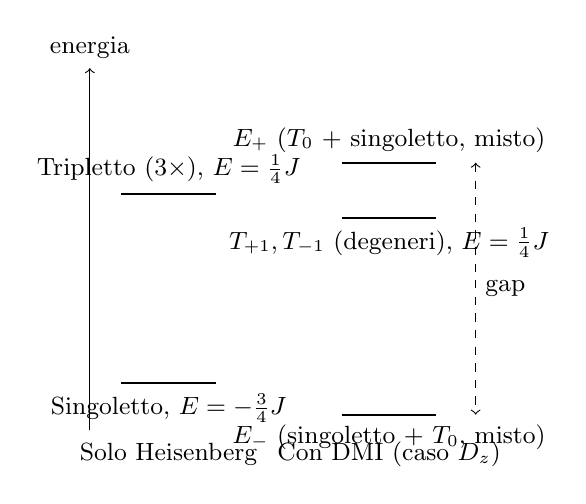
\begin{tikzpicture}[scale=1.0, every node/.style={font=\small}]
 \draw[->] (0,0) -- (0,4.6) node[above]{energia};
 % solo Heisenberg
 \draw[thick] (0.4,3.0) -- (1.6,3.0) node[midway,above]{Tripletto ($3\times$), $E=\frac14 J$};
 \draw[thick] (0.4,0.6) -- (1.6,0.6) node[midway,below]{Singoletto, $E=-\frac34 J$};
 \node at (1.0,-0.3) {Solo Heisenberg};
 % con DMI
 \draw[thick] (3.2,3.4) -- (4.4,3.4) node[midway,above]{$E_+$ ($T_0$ + singoletto, misto)};
 \draw[thick] (3.2,2.7) -- (4.4,2.7) node[midway,below]{$T_{+1},T_{-1}$ (degeneri), $E=\frac14 J$};
 \draw[thick] (3.2,0.2) -- (4.4,0.2) node[midway,below]{$E_-$ (singoletto + $T_0$, misto)};
 \node at (3.8,-0.3) {Con DMI (caso $D_z$)};
 \draw[<->,dashed] (4.9,3.4) -- (4.9,0.2) node[midway,right]{gap};
\end{tikzpicture}
\captionof{figure}{Effetto della DMI (solo $D_z$) sullo spettro energetico: la
degenerazione a tre livelli del tripletto si divide in un livello doppio (invariato,
$T_{\pm1}$) e un livello singolo ($T_0$), che si allontana dal singoletto per
repulsione dei livelli, allargando il gap energetico (rappresentazione qualitativa,
non in scala).}
\end{center}

\paragraph{Apertura del gap energetico.} In un sistema antiferromagnetico ($J>0$), dove
il singoletto \`e lo stato fondamentale, la DMI spinge il singoletto ancora pi\`u in
basso e il tripletto $M=0$ pi\`u in alto: la DMI allarga dunque il gap energetico (spin
gap) fra lo stato fondamentale e la prima eccitazione del sistema.

\section{Stato fondamentale perturbato e angolo di inclinazione (canting angle)}

Per calcolare esplicitamente l'effetto fisico del mescolamento, determiniamo
l'autovettore dello stato fondamentale e il conseguente angolo di inclinazione degli
spin, nel caso in cui sia presente l'interazione di Heisenberg ferromagnetica ($J<0$)
insieme alla sola componente $D_z$ della DMI.

\subsection{Riduzione al sottospazio accoppiato}

L'Hamiltoniana ristretta al sottospazio $\{|0,0\rangle,|1,0\rangle\}$ si riduce alla
matrice $2\times2$
$$H = \begin{pmatrix} -\frac34 J & -\dfrac{iD_z}{2} \\[6pt] \dfrac{iD_z}{2} & \frac14 J \end{pmatrix}.$$

\subsection{Autovalori}

Risolvendo l'equazione secolare $\det(H-\lambda I)=0$,
$$\Big(-\frac34 J-\lambda\Big)\Big(\frac14 J-\lambda\Big) - \Big(\frac{iD_z}{2}\Big)\Big(-\frac{iD_z}{2}\Big) = 0 \;\Longrightarrow\; \lambda^2+\frac12 J\lambda-\frac{3}{16}J^2-\frac14 D_z^2=0,$$
si ottengono le due energie perturbate
$$\lambda_\pm = -\frac14 J \pm \sqrt{\frac14 J^2 + \frac14 D_z^2}.$$

\subsection{Stato fondamentale perturbato}

Assumendo che la DMI sia una piccola perturbazione rispetto allo scambio principale
($|D_z|\ll|J|$), sviluppiamo al primo ordine lo stato fondamentale. Nel caso
ferromagnetico ($J<0$) lo stato imperturbato di partenza \`e il tripletto
$|1,0\rangle$; applicando la teoria delle perturbazioni al primo ordine,
$$|\psi_0\rangle \approx |1,0\rangle + \frac{\langle0,0|H_{\rm DMI}|1,0\rangle}{E_T^{(0)}-E_S^{(0)}}\,|0,0\rangle.$$
Sostituendo l'elemento di matrice $\langle0,0|H_{\rm DMI}|1,0\rangle=-iD_z/2$ e la
differenza di energia imperturbata $\Delta E = \tfrac14 J-(-\tfrac34 J)=J$,
$$|\psi_0\rangle \approx |1,0\rangle - i\,\frac{D_z}{2J}\,|0,0\rangle.$$
Normalizzando lo stato (trattenendo i termini fino al primo ordine in $D_z/J$),
$$|\psi_0\rangle = \frac1{\sqrt{1+\big(\tfrac{D_z}{2J}\big)^2}}\left[|1,0\rangle - i\,\frac{D_z}{2J}\,|0,0\rangle\right].$$

\subsection{Angolo di inclinazione}

Per visualizzare geometricamente l'inclinazione nel piano trasversale $xy$, esprimiamo
lo stato fondamentale nella base computazionale $\{|\!\uparrow\downarrow\rangle,|\!\downarrow\uparrow\rangle\}$
sostituendo le definizioni di singoletto e tripletto:
$$|\psi_0\rangle = \frac1{\sqrt2}\left[\Big(1-i\frac{D_z}{2J}\Big)|\!\uparrow\downarrow\rangle + \Big(1+i\frac{D_z}{2J}\Big)|\!\downarrow\uparrow\rangle\right].$$
Utilizzando l'approssimazione per piccoli angoli $1\pm i\theta\approx e^{\pm i\theta}$,
con $\theta=D_z/(2J)$, lo stato diventa
$$|\psi_0\rangle \approx \frac1{\sqrt2}\Big(e^{-i\theta}|\!\uparrow\downarrow\rangle + e^{i\theta}|\!\downarrow\uparrow\rangle\Big).$$
Questa sfasatura quantistica fra le componenti si traduce direttamente in una
rotazione spaziale degli spin nel piano orizzontale: calcolando i valori di
aspettazione delle componenti di spin per ciascun sito, si dimostra che il primo spin
punta lungo la direzione individuata dall'angolo $-\theta$, il secondo lungo l'angolo
$+\theta$. L'angolo totale di inclinazione relativa fra i due vettori di spin \`e
dunque
$$\alpha = 2\theta = \frac{D_z}{J}.$$
L'interazione antisimmetrica modifica quindi lo stato fondamentale introducendo un
termine immaginario proporzionale a $D_z/(2J)$: gli spin smettono di essere
perfettamente collineari e si inclinano nel piano di un angolo relativo
$\alpha\approx D_z/J$ (in radianti).

\begin{center}
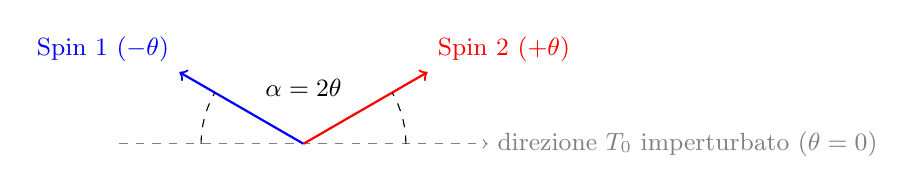
\begin{tikzpicture}[scale=1.3, every node/.style={font=\small}]
 \draw[->,dashed,gray] (-1.8,0) -- (1.8,0) node[right]{direzione $T_0$ imperturbato ($\theta=0$)};
 \draw[->,thick,blue] (0,0) -- (150:1.4) node[above left]{Spin 1 ($-\theta$)};
 \draw[->,thick,red] (0,0) -- (30:1.4) node[above right]{Spin 2 ($+\theta$)};
 \draw[dashed] (180:1.0) arc (180:150:1.0);
 \draw[dashed] (0:1.0) arc (0:30:1.0);
 \draw (90:0.55) node{$\alpha=2\theta$};
\end{tikzpicture}
\captionof{figure}{Rappresentazione geometrica (schematica, angolo $\theta$ esagerato
per chiarezza) dell'inclinazione degli spin nel piano trasversale: a $D_z=0$ i due spin
sono paralleli lungo la direzione del tripletto $T_0$; la DMI li ruota simmetricamente
di $\mp\theta=\mp D_z/(2J)$, separandoli di un angolo relativo $\alpha=2\theta$.}
\end{center}

\section{Geometria vettoriale della DMI: il ruolo dell'asse individuato da $\vec D$}

Nei calcoli precedenti si \`e scelto arbitrariamente un asse di quantizzazione, di
solito l'asse $z$: se il vettore $\vec D$ punta proprio lungo $z$, la componente
modificata \`e il tripletto con $M=0$. \`E istruttivo guardare il problema in modo
puramente geometrico, senza legarsi agli assi coordinati.

Il vettore $\vec D$ definisce una direzione unica nello spazio, che possiamo chiamare
l'asse della DMI. Rispetto a questo asse:
\begin{itemize}
\item lo stato di singoletto si accoppia esclusivamente con lo stato di tripletto che
ha proiezione di spin nulla lungo $\vec D$ (il tripletto $M_{\vec D}=0$), che \`e
proprio la combinazione simmetrica considerata sopra; la sua energia viene alzata (o
comunque modificata) per repulsione dei livelli;
\item gli altri due stati del tripletto (quelli con $M_{\vec D}=\pm1$ rispetto a $\vec
D$) sono completamente ortogonali e non risentono affatto dell'interazione.
\end{itemize}
Poich\'e l'Hamiltoniana di Heisenberg d\`a a tutti e tre i tripletti la stessa energia
$\tfrac14 J$, e la DMI perturba solo uno di essi, gli altri due non cambiano energia e
restano rigorosamente degeneri fra loro. Lo spettro complessivo dei quattro stati, in
presenza di DMI, si divide sempre in: un livello singolo (lo stato fondamentale
modificato, a forte carattere di singoletto), un livello singolo (la combinazione
simmetrica del tripletto sollevata o spostata) e un livello doppiamente degenere (gli
altri due stati del tripletto, rimasti intatti). La DMI, agendo lungo una sola
direzione vettoriale, non ha dunque la forza di distruggere da sola l'intera
degenerazione del tripletto: i due stati perpendicolari a quella direzione restano
protetti da una degenerazione residua a due volte.

\subsection{Perch\'e non \`e possibile isolare un solo stato $M=\mp1$}

Ci si pu\`o chiedere se sia possibile orientare $\vec D$ in modo da lasciare degeneri,
ad esempio, gli stati $|1,-1\rangle$ e $|1,0\rangle$ (definiti rispetto all'asse $z$
iniziale), isolando soltanto $|1,1\rangle$.

\paragraph{Motivo matematico.} Riprendendo la matrice completa, le energie diagonali
dei tre tripletti valgono inizialmente tutte $\tfrac14 J$. La DMI introduce elementi
fuori diagonale che collegano il singoletto $|0,0\rangle$ a questi tripletti,
spostandone l'energia. Per lasciare $|1,-1\rangle$ e $|1,0\rangle$ degeneri alla loro
energia originale, la DMI non dovrebbe toccare nessuno dei due:
\begin{itemize}
\item la componente $D_z$ accoppia il singoletto a $|1,0\rangle$, quindi occorrerebbe
$D_z=0$;
\item le componenti $D_x$ e $D_y$ accoppiano il singoletto simultaneamente a
$|1,1\rangle$ e $|1,-1\rangle$ tramite i termini $(D_x\pm iD_y)$, quindi occorrerebbe
anche $D_x=0$ e $D_y=0$.
\end{itemize}
Annullando tutte le componenti si ottiene $\vec D=0$, cio\`e si spegne completamente la
DMI: non esiste dunque nessuna orientazione di $\vec D$ che realizzi questa particolare
configurazione di degenerazione.

\paragraph{Motivo fisico.} La DMI \`e governata dal prodotto vettoriale $\vec
S_1\times\vec S_2$, che agisce fisicamente come un operatore di transizione di momento
angolare. Le componenti nel piano ($D_x,D_y$) scambiano pacchetti di momento angolare
pari a $\Delta M=\pm1$, associando sempre lo stato a momento nullo ($M=0$) con gli
stati a momento massimo o minimo ($M=\pm1$) in modo perfettamente simmetrico. Non
esiste alcuna inclinazione nello spazio tridimensionale capace di rompere la simmetria
fra $M=+1$ e $M=-1$ isolando soltanto uno dei due, perch\'e l'asse $z$ scelto per
definire quei numeri quantici impone che $M=+1$ e $M=-1$ siano le due facce speculari
della stessa rotazione (oraria e antioraria) attorno a $z$.

\subsection{Le uniche due configurazioni possibili}

In presenza di DMI si possono ottenere solo due tipi di spettro per il tripletto:
\begin{itemize}
\item se $\vec D$ \`e lungo $z$ ($D_x=D_y=0$, $D_z\neq0$): restano degeneri
$|1,1\rangle$ e $|1,-1\rangle$, mentre $|1,0\rangle$ viene isolato e alzato in
energia;
\item se $\vec D$ giace nel piano $xy$ ($D_z=0$): $|1,0\rangle$ resta fermo alla sua
energia originale, mentre $|1,1\rangle$ e $|1,-1\rangle$ si mescolano fra loro,
rompendo la propria degenerazione.
\end{itemize}
L'accoppiamento asimmetrico che lascerebbe degeneri, ad esempio, $M=-1$ e $M=0$
rompendo la simmetria con $M=+1$ non \`e realizzabile con la sola DMI: \`e invece
l'effetto tipico di un campo magnetico esterno (effetto Zeeman) lungo $z$, che separa
linearmente i livelli in base al segno di $M$. Va per\`o notato che se l'effetto
Zeeman \`e presente formalmente nell'Hamiltoniana ma il campo esterno \`e nullo,
$$H_{\rm Zeeman} = -g\mu_B\vec B\cdot\vec S = 0 \qquad (\vec B=0),$$
il termine svanisce completamente, e si ritorna esattamente al caso geometrico
determinato unicamente dal vettore $\vec D$ della DMI.

\subsection{Diagonalizzazione esatta per $\vec D$ generico}

I due casi limite analizzati sopra ($\vec D$ lungo $z$, oppure $\vec D$ nel piano
$xy$) sono in realt\`a un unico risultato, se si ragiona in termini puramente
geometrici anzich\'e in termini delle componenti cartesiane $D_x,D_y,D_z$. La scelta
dell'asse $z$ come asse di quantizzazione per costruire gli stati $|S,M\rangle$ \`e
infatti arbitraria: \`e una scelta di base per descrivere lo spazio di Hilbert, non
una propriet\`a fisica del sistema, e gli autovalori dell'Hamiltoniana non possono
dipendere da essa.

Conviene allora scegliere l'asse di quantizzazione allineato con la direzione fisica
del vettore $\vec D$ stesso. In questa base ruotata, per costruzione, $\vec D$ ha
soltanto la componente lungo il nuovo asse $z'$, di modulo
$$|\vec D| = \sqrt{D_x^2+D_y^2+D_z^2},$$
e il problema si riduce esattamente al caso solo $D_z$ gi\`a risolto, con la
sostituzione $D_z\to|\vec D|$. Gli autovalori esatti della matrice $4\times4$
completa, per un vettore $\vec D$ del tutto generico, sono dunque:
$$E_{T,\perp} = \frac14 J \qquad \text{(doppiamente degenere: i due tripletti con proiezione } \pm1 \text{ lungo } \vec D\text{)},$$
$$E_\pm = -\frac14 J \pm \sqrt{\frac14 J^2 + \frac14|\vec D|^2} \qquad \text{(singoletto e tripletto con proiezione nulla lungo } \vec D\text{, mescolati)}.$$
Allo stesso modo, l'angolo di canting ricavato in precedenza si generalizza a
$$\alpha \approx \frac{|\vec D|}{J} \qquad (|\vec D|\ll|J|),$$
con il piano di inclinazione degli spin determinato dalla direzione trasversale di
$\vec D$ rispetto all'asse $z'$ cos\`i definito. Questo risultato conferma in forma
chiusa quanto argomentato geometricamente sopra: qualunque sia l'orientazione di
$\vec D$, lo spettro consiste sempre di un livello doppiamente degenere e di una
coppia di livelli mescolati per repulsione, mai di una rottura completa e indipendente
delle tre degenerazioni del tripletto.

\part{Oltre il sistema isolato: origine microscopica, anisotropia e mappatura su qubit}

\section{Origine microscopica di $J$ e $\vec D$: superscambio e regole di Moriya}

Le costanti $J$ e $\vec D$ che compaiono nell'Hamiltoniana non sono parametri liberi:
hanno un'origine microscopica ben precisa, che vale la pena richiamare brevemente per
completare il quadro fisico.

\paragraph{Origine di $J$: il superscambio.} In un isolante magnetico, lo scambio
diretto tra due ioni magnetici \`e tipicamente troppo debole, perch\'e le loro
funzioni d'onda si sovrappongono poco. Il meccanismo dominante \`e invece il
superscambio (meccanismo di Anderson): gli elettroni compiono un salto virtuale
attraverso gli orbitali di uno ione non magnetico interposto (tipicamente un ligando
come $\mathrm{O}^{2-}$), e il principio di esclusione di Pauli, applicato a questo
processo virtuale, genera un accoppiamento effettivo tra gli spin dei due ioni
magnetici. Il segno e l'intensit\`a di $J$ dipendono in modo sensibile dalla geometria
del legame -- in particolare dall'angolo ione--ligando--ione -- secondo le regole
qualitative di Goodenough--Kanamori: legami a $\sim180^\circ$ tra orbitali
semi-occupati tendono a dare un accoppiamento antiferromagnetico forte ($J>0$),
mentre legami a $\sim90^\circ$ tendono a dare un accoppiamento ferromagnetico pi\`u
debole ($J<0$).

\paragraph{Origine di $\vec D$: spin-orbita e le regole di Moriya.} L'interazione di
Dzyaloshinskii--Moriya fu introdotta inizialmente in forma fenomenologica da
Dzyaloshinskii (1958), tramite argomenti di simmetria nello spirito della teoria di
Landau, per spiegare il debole ferromagnetismo osservato in antiferromagneti come
l'ematite. Moriya (1960) ne fornì poi una derivazione microscopica, mostrando che la
DMI emerge come la correzione dominante al superscambio dovuta all'accoppiamento
spin-orbita sullo ione magnetico: \`e, in questo senso, un effetto del primo ordine
nella costante di accoppiamento spin-orbita (mentre i termini di scambio anisotropo
simmetrico, discussi pi\`u avanti, sono effetti del second'ordine).

Moriya stabil\`i inoltre un insieme di regole di simmetria che vincolano la direzione
permessa di $\vec D_{12}$ a partire dalla simmetria puntuale locale del legame che
unisce i siti 1 e 2 (le cosiddette regole di Moriya):
\begin{itemize}
\item se esiste un centro di inversione nel punto medio del legame, $\vec D=0$
(coerentemente con quanto visto in precedenza: la DMI richiede l'assenza di simmetria
di inversione);
\item se un piano speculare perpendicolare al legame passa per il suo punto medio,
$\vec D$ giace in quel piano;
\item se un piano speculare contiene entrambi i siti, $\vec D$ \`e perpendicolare a
quel piano;
\item se un asse di rotazione binario perpendicolare al legame passa per il suo punto
medio, $\vec D$ \`e perpendicolare a tale asse;
\item se un asse di rotazione $n$-ario ($n\geq2$) \`e diretto lungo il legame, $\vec
D$ \`e parallelo al legame stesso.
\end{itemize}
Queste regole spiegano perch\'e, in un dato materiale, il vettore $\vec D$ non possa
puntare in una direzione arbitraria, ma sia vincolato dalla geometria cristallina
specifica del composto in esame.

\section{Anisotropia di scambio e limiti del modello isotropo}

Un punto delicato merita una precisazione esplicita, perch\'e riguarda la validit\`a
stessa di un termine spesso invocato per rimuovere la degenerazione residua a due
livelli lasciata dalla sola DMI.

\paragraph{Perch\'e l'anisotropia a singolo ione non si applica qui.} Per un sito con
spin 1/2, la componente $S_{iz}$ ha soltanto gli autovalori $\pm\tfrac12$, quindi
$(S_{iz})^2=\tfrac14 I$ su ogni stato, senza eccezioni. Un termine di anisotropia a
singolo ione della forma $-D_{\rm an}\big[(S_{1z})^2+(S_{2z})^2\big]$ \`e dunque, per
due spin 1/2, semplicemente una costante additiva: non distingue in alcun modo gli
stati con $M=0$ da quelli con $M=\pm1$, e non pu\`o produrre lo splitting che le si
vorrebbe attribuire. Questo tipo di anisotropia cristallina \`e fisicamente reale e
importante, ma soltanto per ioni con spin $S\geq1$ (ad esempio $\mathrm{Ni}^{2+}$,
$S=1$, o $\mathrm{Fe}^{3+}$, $S=5/2$), per i quali $(S_{iz})^2$ assume effettivamente
valori diversi al variare di $M$.

\paragraph{Il meccanismo corretto per spin 1/2: l'anisotropia di scambio.} Per un
dimero di spin 1/2, l'analogo fisicamente corretto \`e invece un termine di scambio
anisotropo (un'Hamiltoniana di tipo XXZ),
$$H_{XXZ} = J_x S_{1x}S_{2x} + J_y S_{1y}S_{2y} + J_z S_{1z}S_{2z}, \qquad J_x=J_y\equiv J\neq J_z,$$
esattamente la stessa struttura del modello anisotropo a dimero $H=J_x X_1X_2+J_y
Y_1Y_2+J_z Z_1Z_2+b(Z_1+Z_2)$ (con $S_i=\vec\sigma_i/2$). Isolando lo scarto
$\Delta J\equiv J_z-J$ rispetto alla parte isotropa gi\`a inclusa in $H_{\rm sym}$, si
ha un termine aggiuntivo $\Delta J\,S_{1z}S_{2z}$. Poich\'e $S_{1z}S_{2z}$ \`e
diagonale nella base computazionale, con autovalore $+\tfrac14$ su
$|\!\uparrow\uparrow\rangle,|\!\downarrow\downarrow\rangle$ e $-\tfrac14$ su
$|\!\uparrow\downarrow\rangle,|\!\downarrow\uparrow\rangle$, esso \`e automaticamente
diagonale anche sulla base $\{S,M\}$ (poich\'e non mescola $|\!\uparrow\downarrow\rangle$
e $|\!\downarrow\uparrow\rangle$):
$$\langle1,\pm1|S_{1z}S_{2z}|1,\pm1\rangle = +\frac14, \qquad \langle1,0|S_{1z}S_{2z}|1,0\rangle=\langle0,0|S_{1z}S_{2z}|0,0\rangle=-\frac14.$$
Aggiungendo $\Delta J\,S_{1z}S_{2z}$ all'Hamiltoniana isotropa, le energie diventano
$$E_{T,\pm1}=\frac14 J+\frac{\Delta J}{4}, \qquad E_{T,0}=\frac14 J-\frac{\Delta J}{4}, \qquad E_S=-\frac34 J-\frac{\Delta J}{4}.$$
Per $\Delta J\neq0$, i due stati $M=\pm1$ restano degeneri fra loro ma si separano
nettamente dal tripletto $M=0$: lo stesso obiettivo qualitativo che ci si proponeva con
l'anisotropia a singolo ione, ma ottenuto con un meccanismo fisicamente valido per spin
1/2.

\paragraph{Combinare anisotropia di scambio e DMI nel piano.} Se si accende anche la
componente nel piano della DMI ($D_x,D_y$) insieme a questo termine $\Delta
J\,S_{1z}S_{2z}$, le componenti nel piano mescolano e sollevano lo stato $|1,1\rangle$
(e $|1,-1\rangle$), mentre $|1,0\rangle$ resta fisso all'energia sopra calcolata.
Bilanciando finemente $\Delta J$ e $(D_x,D_y)$ \`e possibile far s\`i che uno dei due
livelli risultanti dal mescolamento di $|1,\pm1\rangle$ incroci esattamente l'energia
di $|1,0\rangle$, realizzando cos\`i, a campo magnetico nullo, configurazioni di
(quasi-)degenerazione altrimenti irraggiungibili con la sola DMI.

\section{Un esempio numerico: ordini di grandezza realistici}

Per dare concretezza alle formule precedenti \`e utile un esempio numerico, con
l'avvertenza che i valori usati qui sono puramente illustrativi (dell'ordine di
grandezza tipico riportato in letteratura per sistemi con debole ferromagnetismo
indotto da DMI, come l'ematite $\alpha$-$\mathrm{Fe}_2\mathrm{O}_3$, il silicide di
manganese $\mathrm{MnSi}$, il borato di ferro $\mathrm{FeBO}_3$ o gli ortoferriti
$\mathrm{RFeO}_3$): in questi materiali le costanti di superscambio sono tipicamente
dell'ordine di $J\sim1$--$10$~meV, mentre il vettore DMI, essendo un effetto del primo
ordine in spin-orbita anzich\'e di scambio diretto, \`e tipicamente un ordine di
grandezza pi\`u piccolo, con rapporti $D/J\sim10^{-2}$--$10^{-1}$.

Prendendo valori illustrativi $J=10$~meV e $D_z=1$~meV (cio\`e $D_z/J=0.1$), le
formule ricavate in precedenza danno:
$$\theta = \frac{D_z}{2J} = 0.05\ {\rm rad}, \qquad \alpha = 2\theta \approx 0.1\ {\rm rad}\approx5.73^\circ,$$
per l'angolo di canting, e per i livelli perturbati
$$\lambda_+ = -\frac{J}{4}+\sqrt{\frac{J^2}{4}+\frac{D_z^2}{4}} = -2.5+\sqrt{25+0.25}\approx2.52\ {\rm meV} \quad (\text{contro } E_T=2.5\ {\rm meV\ imperturbato}),$$
$$\lambda_- = -\frac{J}{4}-\sqrt{\frac{J^2}{4}+\frac{D_z^2}{4}} \approx -7.52\ {\rm meV} \quad (\text{contro } E_S=-7.5\ {\rm meV\ imperturbato}),$$
in buon accordo con la stima perturbativa $\delta E\approx D_z^2/(4J)=0.025$~meV.
Questo esercizio mostra che, anche con un rapporto $D/J$ relativamente piccolo (il
regime tipico dei materiali reali), l'angolo di canting risultante non \`e affatto
trascurabile: pochi gradi di inclinazione sono sufficienti a generare un momento
ferromagnetico netto misurabile in un antiferromagnete altrimenti collineare. Per un
materiale specifico, \`e naturalmente necessario sostituire questi valori illustrativi
con $J$ e $D$ estratti da misure sperimentali o da calcoli \emph{ab initio}.

\section{Mappatura su operatori di Pauli e rilevanza per il calcolo quantistico}

Poich\'e $\vec S_i=\tfrac12\vec\sigma_i$, le componenti del prodotto vettoriale che
definiscono la DMI si riscrivono immediatamente in termini di operatori di Pauli a due
qubit:
$$(\vec S_1\times\vec S_2)_z = \frac14(X_1Y_2-Y_1X_2), \qquad (\vec S_1\times\vec S_2)_x = \frac14(Y_1Z_2-Z_1Y_2), \qquad (\vec S_1\times\vec S_2)_y = \frac14(Z_1X_2-X_1Z_2),$$
da cui
$$H_{\rm DMI} = \frac{D_x}{4}(Y_1Z_2-Z_1Y_2) + \frac{D_y}{4}(Z_1X_2-X_1Z_2) + \frac{D_z}{4}(X_1Y_2-Y_1X_2).$$
Ciascuno di questi termini \`e una somma di due stringhe di Pauli a due qubit,
esattamente della stessa natura dei termini $J_xX_1X_2$, $J_yY_1Y_2$, $J_zZ_1Z_2$ che
compaiono nel modello anisotropo del dimero: la loro implementazione su circuito (ad
esempio all'interno di un ansatz VQE o di una decomposizione di Trotter) richiede
soltanto gli stessi cambi di base a singolo qubit e le stesse porte entanglizzanti a
due qubit gi\`a impiegate per i termini di Heisenberg, applicati alle combinazioni
$X_1Y_2$ e $Y_1X_2$ anzich\'e a $X_1X_2$ o $Y_1Y_2$. \`E interessante notare che, a
livello della decomposizione in operatori di Pauli, la struttura
simmetrica/antisimmetrica discussa in tutto questo documento si manifesta di nuovo: i
termini di Heisenberg accoppiano ciascun asse a se stesso ($X_1X_2$, $Y_1Y_2$), mentre
i termini DMI accoppiano assi diversi in combinazione antisimmetrica ($X_1Y_2-Y_1X_2$,
e cicliche). Aggiungere un termine DMI a un modello di dimero gi\`a implementato non
richiede quindi nuovi elementi concettuali dal punto di vista della simulazione
quantistica, ma soltanto ulteriori termini nella stessa famiglia di stringhe di Pauli a
due qubit.

\section{Cenni: estensione a pi\`u spin e chiralit\`a nelle strutture ad anello}

Quanto discusso finora riguarda il caso di due soli spin. Su topologie con $N\geq3$
siti -- come una catena aperta o un anello triangolare -- compare un fenomeno
qualitativamente nuovo, che qui si accenna soltanto senza svolgerlo in dettaglio.

Su un anello di tre spin, la DMI \`e definita su ciascun legame separatamente, con
vettori $\vec D_{12}$, $\vec D_{23}$, $\vec D_{31}$. Se questi tre vettori sono legati
dalla simmetria di rotazione a $120^\circ$ dell'anello (ciascuno ruotato rispetto al
precedente seguendo la simmetria del ciclo), il loro effetto combinato non si limita
pi\`u a un semplice canting locale bond-per-bond: pu\`o stabilizzare una chiralit\`a
scalare netta,
$$\chi = \vec S_1\cdot(\vec S_2\times\vec S_3),$$
una quantit\`a dispari per inversione temporale e per parit\`a, ma invariante per
permutazione ciclica dei tre siti. In altre parole, anche se ciascun singolo legame
rompe poca simmetria (un $\vec D_{ij}$ piccolo rispetto a $J$), la somma coerente di
tre rotture di simmetria disposte lungo un anello chiuso pu\`o generare un ordine
magnetico genuinamente non collineare e chirale, che non ha analogo nel caso a due
soli spin discusso in questo documento. \`E questo il meccanismo microscopico alla
base delle tessiture di spin a elica (\emph{proper-screw}) osservate in
antiferromagneti triangolari e in reticoli kagome. Una trattazione quantitativa di
questo effetto per le topologie $N=3$ (catena aperta e anello/triangolo) richiederebbe
la diagonalizzazione esplicita dell'Hamiltoniana a tre corpi, che esula dallo scopo di
queste note ma costituisce una naturale direzione di approfondimento.

\section{Conclusioni}

Lo studio della simmetria e dell'antisimmetria per scambio di due spin 1/2 mostra come
queste due propriet\`a, apparentemente astratte, determinino in modo diretto la
geometria delle configurazioni magnetiche possibili:
\begin{itemize}
\item la componente simmetrica (Heisenberg, $J\vec S_1\cdot\vec S_2$) favorisce
configurazioni collineari, con lo stato fondamentale interamente determinato dal
segno di $J$ (singoletto per $J>0$, tripletto per $J<0$);
\item la componente antisimmetrica (DMI, $\vec D\cdot(\vec S_1\times\vec S_2)$) agisce
come un ponte selettivo fra singoletto e tripletto, dettato univocamente
dall'orientazione del vettore $\vec D$: scegliendo l'asse di quantizzazione lungo
$\vec D$, il problema si riduce sempre a un'unica coppia di livelli mescolati (di
modulo $|\vec D|/2$) pi\`u una coppia di tripletti che restano degeneri;
\item questo mescolamento produce stati fondamentali misti, inclina gli spin di un
angolo $\alpha\approx|\vec D|/J$, e rimuove parzialmente -- mai completamente da sola
-- la degenerazione del tripletto, lasciando sempre una degenerazione residua a due
livelli;
\item la rimozione completa di questa degenerazione residua a campo magnetico nullo
richiede un ulteriore ingrediente fisico: per spin 1/2, non l'anisotropia a singolo
ione (che per $S=1/2$ \`e una costante additiva priva di effetto), bens\`i
l'anisotropia di scambio ($J_z\neq J_x=J_y$, un termine XXZ), in combinazione con la
componente nel piano della DMI;
\item entrambe le costanti $J$ e $\vec D$ hanno un'origine microscopica precisa
(superscambio e regole di Moriya, rispettivamente), che vincola sia il segno di $J$
sia la direzione permessa di $\vec D$ alla geometria cristallina del materiale;
\item la stessa struttura simmetrica/antisimmetrica si ritrova, identica, nella
decomposizione in operatori di Pauli rilevante per la simulazione quantistica del
sistema, e si arricchisce di fenomeni qualitativamente nuovi (chiralit\`a scalare) non
appena si passa da due a tre o pi\`u spin.
\end{itemize}

Il quadro complessivo che ne emerge \`e quello di una gerarchia di interazioni --
scambio isotropo, DMI, anisotropia di scambio, ed eventualmente un campo Zeeman
esterno -- ciascuna delle quali agisce con una propria regola di simmetria selettiva
sugli stessi quattro stati di base (un singoletto e tre tripletti), costruendo
progressivamente lo spettro energetico completo e le propriet\`a geometriche
(collineari, canted, chirali) del sistema di spin.

\appendix
\section{Verifica numerica: codice di calcolo degli elementi di matrice}

Gli elementi di matrice ricavati analiticamente nella Parte~I possono essere verificati
costruendo esplicitamente gli operatori di spin come matrici di Pauli (opportunamente
normalizzate) e calcolando le componenti del prodotto vettoriale $\vec S_1\times\vec
S_2$ nella base $\{\text{Singoletto},T_+,T_0,T_-\}$. Lo script seguente, basato su
\texttt{numpy}, riproduce il calcolo:

{\small
\begin{verbatim}
import numpy as np

# Matrici di spin 1/2
Sx = 0.5 * np.array([[0, 1], [1, 0]])
Sy = 0.5 * np.array([[0, -1j], [1j, 0]])
Sz = 0.5 * np.array([[1, 0], [0, -1]])
I = np.eye(2)

# Operatori di spin sui due siti
S1x = np.kron(Sx, I)
S1y = np.kron(Sy, I)
S1z = np.kron(Sz, I)

S2x = np.kron(I, Sx)
S2y = np.kron(I, Sy)
S2z = np.kron(I, Sz)

# Componenti del prodotto vettoriale
Vz = S1x @ S2y - S1y @ S2x
Vx = S1y @ S2z - S1z @ S2y
Vy = S1z @ S2x - S1x @ S2z

# Stati: base |up up>, |up down>, |down up>, |down down>
t_plus  = np.array([1, 0, 0, 0])
t_minus = np.array([0, 0, 0, 1])
t_zero  = np.array([0, 1, 1, 0]) / np.sqrt(2)
singlet = np.array([0, 1, -1, 0]) / np.sqrt(2)

basis = [singlet, t_plus, t_zero, t_minus]
names = ['Singlet', 'Triplet+', 'Triplet0', 'Triplet-']

for label, V in [('Vz', Vz), ('Vx', Vx), ('Vy', Vy)]:
    print(f"\n{label} matrix elements:")
    for i, b1 in enumerate(basis):
        for j, b2 in enumerate(basis):
            val = b1.conj().T @ V @ b2
            if np.abs(val) > 1e-5:
                print(f"  <{names[i]}|{label}|{names[j]}> = {val}")
\end{verbatim}
}

Il risultato di questo calcolo conferma quanto ricavato analiticamente: la componente
$V_z=(\vec S_1\times\vec S_2)_z$ presenta elementi di matrice non nulli soltanto fra il
singoletto e il tripletto $M=0$, con modulo $|D_z|/2$ per un accoppiamento $D_z$
generico, mentre le componenti $V_x$ e $V_y$ presentano elementi non nulli soltanto tra
il singoletto e i tripletti $M=\pm1$, con modulo $|D_\perp|/(2\sqrt2)$ -- coerentemente
con la struttura della matrice hamiltoniana completa discussa in \S11.3 e con la
richiesta di isotropia $\|(\vec S_1\times\vec S_2)_a|0,0\rangle\|=1/2$ per $a=x,y,z$
(§9.3, §10).

\end{document}
